\documentclass{article}

\usepackage{url}
\usepackage{fontspec}
\usepackage{graphicx}
\graphicspath{ {img/} }

%\usepackage{e-tex}
%\usepackage{etoolbox}
%\usepackage{keyval}
%\usepackage{ifthen}
%\usepackage[czech]{babel}
%\usepackage[backend=biber]{biblatex}
%\usepackage{biblatex}
%\usepackage{polyglossia}
%\usepackage[autostyle]{csquotes}
%\setmainlanguage{english}
%\usepackage{microtype}
%\usepackage[authordate15, backend=biber]{biblatex-chicago}
%\addbibresource{bibl.bib}



\begin{document}

\tableofcontents

\section{Úvod}

Cílem této práce je popsat možná zadávání textu, rozebrat jejich positiva a negativa a ukázat praktickou implementaci jednoho řešení implementujícího prediktivní text pro webový editor CKEditor.

Teoretická část se bude zabývat historickým vývojem v oblasti prediktivního textu, motivacemi, jež stály za samotným vznikem a rozebere, které z motivací jsou aktuální dodnes a jak se situace v průběhu času změnila. Na základě toho se pak pokusí shrnout základní požadavky na funkce prediktivního textu, zejména v oblasti zadávání textu. 
[/ tady by to jeste neco chtelo /]

Praktická část popíše implementaci prediktivního textu do webového editoru CKEditor. Jako zdroj doplnění využívá tato aplikace data zasílaná vzdáleným serverem. Budou rozebrány použité metody, důvody stojícími za jejich volbou a výhody a nevýhody zvoleného řešení.

\section{Teoretická část}

Prediktivní text, neboli automatické doplňování textu (angl. autocomplete) je funkce v aplikaci, která na základě uživatelského vstupu (většinou prvních několika znaků slova) doplňuje zbytek části textu (většinou slova). V ideálním případě funkce jednoznačně rozpozná, co chtěl uživatel napsat, a nabídne mu právě to doplnění, jež uživatel chce. V praxi obvykle uživatel dostává na výběr z několik možností, které systém vyhodnotil jako nejpravděpodobnější doplnění vstupu. Systémy se liší způsobem zužování výběru možností a jejich řazením, stejně tak jako vizuálním podáním nabídky.

Všechny systémy automatického doplňování textu fungují nejlépe v implementacích na omezených doménách, tzn. například doplňování e-mailových adres v e-mailových klientech, klíčových slov určitého programovacího jazyka v editorech určených k programování či ve formulářových polích s předem vymezeným očekávaným vstupem. 

Systémy pro predikci textu určené k tvorbě volného textu jsou obvykle založeny na více či méně rozsáhlém lokálně uloženém korpusu slov či spojení, ze kterého vybírají možná doplnění. Tyto systémy zpravidla umožňují uživateli přidávat manuálně slova, která napsal a nejsou v základním korpusu, což slouží jako základní uživatelské přizpůsobení. Lokální korpus má ovšem tu nevýhodu, že jeho velikost je značně limitována možnostmi zařízení, tj. jeho paměťovou a výpočetní kapacitou. To je problém především pro jazyky s rozvinutou flexí, jako je čeština, které potřebují na rozdíl analytických jazyků, např. angličtiny, mnohem větší množství tvarů jednotlivých slov. 

Tento poměr lze porovnat například na dvou velkých korpusech, enTenTen13 a czTenTen12. Jde o rozsáhlé korpusy vytvořené z textů získaných na Internetu, které byly vyčištěny a zbaveny duplikátů nástrojem Onion [/ cit. http://corpus.tools/wiki/Onion /] Anglický korpus enTenTen13 obsahuje 39 011 368 slov a 37 065 442 lemmat, což jsou základní slovní tvary. Naproti tomu český korpus czTenTen12 obsahuje slov 18 725 879 a lemmat pouze 13 976 481. 

Tento rozdíl v poměru lemmat a slov ukazuje na relativně zjevý fakt, že v češtině připadá na jedno lemma mnohem více slovních tvarů než v angličtině, jelikož je čeština flektivní jazyk. Tento fakt značně komplikuje implementaci jazykových  modelů do aplikací pro predikci textu, protože v případě slovníkového modelu je nutno uchovávavat značně větší množství slovních tvarů než u angličtiny. Stejně tak je výrazně větší potřeba zohledňovat kontext, aby byly slovní tvary vybírány správně.

[/ tohle je uplne blbe - jednak napsany, jednak ta uvaha je zcestna /]
Poměr slov a lemmat ilustruje rozdíl mezi unikátními slovy v nezákladním tvaru a unikátními slovy v základním tvaru, tedy lemmaty, což lze považovat za základní ukazatel při porovnávání jazyků na průměrné množství různých tvarů od jednoho slova. V češtině tedy podle výše uvedených dat připadá na jedno lemma 1,339 slovního tvaru, naproti tomu v angličtině na jedno lemma připadá pouze 1,052 slovního tvaru. Je tedy vidět, že slovník pro češtinu by v ideálním případě měl být minimálně 1,27× větší než slovník o stejném množství základních tvarů pro angličtinu. [/ to je nejak malo, ne? kdyz si vezmu, ze ke kazdymu plnovyznamovymu slovu je nejakych cca 5-10 tvarů /] [/ cit.: info o korpusech /]
[/ az sem /]

\subsection{Klíčové vlastnosti systému pro predikci textu}

Navzdory velmi odlišným způsobům použití systémů pro doplňování textů jsou některé jejich klíčové vlastnosti pro většinu implementací společné. Studie, které zkoumaly efektivitu těchto systémů, obecně docházejí ke podobným závěrům, co se požadavků na tyto systémy týče. Ať jde o vyhledávač typu Google nebo Yahoo, o našeptávač e-mailových adres v e-mailovém klientu nebo o predikci volného textu v textovém editoru, aby uživatel měl při užívání aplikace pocit, že mu doplňování textu skutečně pomáhá spíše než překáží, je klíčových několik vlastností.  Primární je rychlost, s níž aplikace možná doplnění uživateli zobrazuje. Nandi a Jagadish uvádí, že by odezva neměla převyšovat 100 ms \cite{Nandi2007}. Tento faktor je rozhodující pro to, zda si uživatel zvolí nabídnutá doplnění použít, nebo raději napíše zbytek textu sám. V případě implementace predikce textu do editoru, kde uživatel zadává volný text, jímž si je relativně jist, je tato vlastnost pro uživatelovo rozhodnutí patrně klíčová. Naproti tomu ve vyhledávání lze očekávat, že uživatel bude ochoten počkat delší chvíli na zobrazení doplnění, zvláště v případě, není-li si jist např. tím, jak se vyhledávaný výraz píše. Na volný text toto implementovat z výše uvedených důvodů nelze.  S tímto souvisí i další vlastnost, kterou uvádí Ward a kol. v publikaci Autocomplete as a Research Tool: A Study on Providing Search Suggestions - umožnění uživateli pohodlně nabízené predikce ignorovat. Rozhodne-li se totiž, že např. bude rychlejší text manuálně napsat a predikce nepoužít, je žádoucí, aby grafické zpracování nabídky žádným způsobem neztěžovalo takto učinit. Z tohoto důvodu je ve většině systémů nabídka předvídaných výrazů zobrazována pod textovým polem (např. Google Suggest 
[/ citace? /]
). Zobrazení nabídky v textových editorech, kde se nejedná o jednořádkové pole s očekávaným vstupem pouze několika jednotlivých slov, je předmětem několika studií, z nichž např. jedna navrhuje zobrazovat nabídku na spodní části obrazovky, aby uživatel nebyl nucen přesouvat pozornost příliš daleko od klávesnice 
[/ fuck kde jsem to cetl? citace /]
. Lze ale polemizovat nad tím, jak je tato argumentace validní pro uživatele bez motorického nebo jiného postižení, jelikož tací většinou při psaní na klávesnici nehledí. Textové editory pro psaní programového kódu tento problém většinou řeší zobrazováním nabízených doplnění v menu pod kursorem (tedy zhruba podobně jako jednořádková vyhledávací a jiná pole). Podobně to řeší i kancelářský balík OpenOffice (příp. LibreOffice), který zobrazuje po napsání prvních tří písmen slova jednu predikci nad kursorem. Výběr predikce se odvíjí od frekvence, přičemž velký důraz je kladen na délku nabízeného slova (obrázek \ref{fig:LOpredict} na straně \pageref{fig:LOpredict}). Tento systém uživateli umožňuje udržovat pozornost na relativně malé oblasti obrazovky, čímž se zvyšuje pravděpodobnost, že se rozhodne doplnění použít. 

\begin{figure}[h]
	\caption{Implementace predikce textu v LibreOffice Writer 4.2.8.2}
	\label{fig:LOpredict}
	\centering
	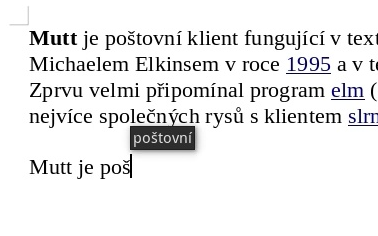
\includegraphics[width=0.7\textwidth]{LO_prediction_1}
\end{figure}

\subsection{Smysl automatického doplňování pro uživatele}

Vedle původního určení predikce textu, kterým je zrychlit zadávání textu a tím komunikaci na rozhraní člověk-počítač, plní pro běžného uživatele automatické doplňování textu ještě několik dalších funkcí. Nejde ani tolik o rychlost zadávání textu, jako spíše o to, co je zadáváno. 

Ward et al. (Autocomplete as a Research Tool) ve své studii uvádí, že studenti, na kterých testoval automatické doplňování ve vyhledávání v rámci informačního systému knihovny, poukázali v následném dotazníku na několik dalších funkcí, které pro ně predikce plnila. 

Na otázku, jak by svým přátelům vysvětlil, k čemu je našeptávač dobrý, odpověděl jeden student, že rozhodně jako asistence v pravopise. Studenti totiž často nemají z ústních zadání v hodinách úplně přesnou představu, jak se např. autor, jehož díla jim jejich vyučující doporučil jako zdroj informací k práci, přesně píše. Autoři studie ze záznamů hledání vyvodili, že někteří studenti si ani nemuseli být vědomi faktu, že začátek jména autora zadali špatně, protože predikce jim nabídla rovnou správnou verzi a oni ji vybrali, aniž by přemýšleli, v čem se nabídka liší od jejich vstupu. 

Mezi další výhody, které studenti uvedli ve výše uvedené studii, patřilo například to, že automatické doplňování jim potvrdilo, že podobné téma již někdo před nimi hledal, a jejich pojetí zpracovávaného tématu je tedy pravděpodobně správné. 

S tímto souvisí i jedna odpověď od dalšího účastníka studie, která uvádí, že autocomplete pro ně fungoval jako nástroj pro dotvoření myšlenky, jako brainstorming od počítače. 

Z výše uvedeného lze tedy vyvozovat, že automatické doplňování textu skutečně nemá význam pouze pro uživatele tělesně či jinak postižené, kteří mohou mít problém se samotným zadáváním textu, ale může posloužit i běžným uživatelům jako nástroj pro kontrolu toho, zda to, co píšou, je správně, k tématu a podobně. [14]

\subsection{Měření účinnosti zadávání textu}

S ohledem na velké množství metod zadávání textu, z nichž mnohé obsahují technologie na ušetření počtu nutných stisků, je nutné mít možnost nějakým objektivním způsobem testovat jednotlivé metody, porovnávat je a zjistit jejich skutečné možnosti. Pro tyto účely slouží metoda výpočtu KSPC (zkratka pro keystrokes per character). Jak název napovídá, udává průměrný počet stisků kláves nutných k zadání jednoho znaku danou metodou\footnote{přestože název obsahuje stisky kláves, veličina se používá i pro měření účinnosti zadávání textu např. pomocí stylusu na dotykovém zařízení}.

Metody zadávání textu lze podle KSPC rozdělit do tří kategorií: ty, pro které je KSPC větší než 1, ty, pro které je rovno 1 a nakonec ty, jejichž KSPC dosahuje hodnot nižších než 1.

Jako základ pro výpočet KSPC pro jednotlivé metody zadávání je vhodná standardní QWERTY klávesnice. Budeme-li uvažovat pouze malá písmena anglické abecedy, platí pro ni, že KSPC = 1, tedy na jeden znak připadá jeden stisk klávesy. Klávesnici QWERTY lze tedy považovat za jednoznačnou metodu zadávání, pro každý znak má jednu dedikovannou klávesu.

Pro další metody zadávání už proces výpočtu tak jednoduchý není a má dva požadavky. Prvním z nich je jednoznačný popis postupu, kterým lze dojít k zadání jednotlivých znaků, druhým je pak jazykový model. Ten je nutný proto, aby výsledné KSPC bylo nezávislé na konkrétním textu v daném jazyce (tedy aby pro daný jazyk bylo průměrné).

\seubsection{Jazykový model}

Jazykovým modelem je v tomto případě korpus a jeho omezené formy. Tyto formy se liší podle toho, jaká metoda zadávání je testována. Pokud například jde o metodu, která vybírá znaky nezávisle na kontextu (na okolních znacích), stačí mít informace o frekvenčním rozložení jednotlivých písmen v korpusu. Pokud by byl výběr znaku závislý na kontextu jednoho písmene, byl by jazykový model frekvenční slovník bi-gramů. Pro delší závislosti MacKenzie et al. (2015) použili frekvenční slovník celých slov.

\subsection{Výpočet KSPC}


\[
	KSPC = \frac{\sum{ (K_c × F_c) }}{\sum{ (C_c × F_c) }}
\]

kde $K_c$ je počet úhozů nutný pro zadání znaku, $C_c$ je velikost znaku a $F_c$ je frekvence daného znaku v korpusu. Pokud se tedy tento vzorec aplikuje na situaci, kdy metoda zadávání textu vybírá písmeno bez ohledu na kontext, platí, že $C_c$ = 1, pokud se vybírá v závislosti na jednom předešlém znaku, je $C_c$ = 2. Pokud metoda zohledňuje celá slova, počítá se s průměrnou délkou slov v daném jazyce. Ta se počítá jako vážený průměr počtu znaků ve slovech daného jazyka, který pro BNC vychází na 4,59 znaku; pro srovnání, [15] počítá při svých výpočtech s 5 úhozy na slovo.


[/ pokud bych potreboval natahovat, tak tady by se klidne dala dat podkapitola "rozdeleni metod vstupu podle KSPC - a vykrast MacKenzieho  /]


\section{Technický bláboly okolo predikce}


Problematika predikce textu je intenzivně zkoumána od dob, kdy se rozšířily mobilní telefony s podporou zadávání textu. Jelikož velikost zařízení od začátku nedovolovala osazení plné QWERTY klávesnice, objevovaly se její náhrady, které jsou podrobněji popsány v dalších kapitolách této práce. Jakkoliv se mohla jejich implementace odlišovat, měly obvykle společnou jednu vlastnost, a to nejednoznačnost. Nejrozšířenější se stala klávesnice typu  [/ nejaky to oznaceni, ATX? /], která se udržela dodnes. Tento typ klávesnice sdružuje písmena po třech až čtyřech na jednu klávesu, přičemž ze skupiny se pak vybírá v základním režimu pomocí opakovaných stisků kláves (multitap). Vzhledem k velmi zásadním omezením rychlosti, které tento způsob zadávaní implikuje, byly vyvinuty různé technologie, které se snažily o zrychlení zadávání tak, aby KSPC bylo rovno jedné nebo ideálně menší jedné.

Aby bylo dosaženo KSPC rovného jedné, stačí technologie typu T9, která vyhledává ve slovníku možné kombinacee písmen ze stisknutých kláves a nalezené pak předkládá uživateli. V případě, že existuje ve slovníku pouze jedno slovo, které odpovídá kombinaci písmen ze stisknutých kláves, je dosaženo KSPC rovného jedné. Pokud však takových slov ve slovníku existuje více, je nutno provést výběr a jeho potvrzení, což zvyšuje KSPC nad jedna.

Pro dosažení hodnot KSPC nižších než jedna je už nutné implementovat predikci textu. To znamená, že aplikace musí uhádnout psané slovo ještě dříve, než uživatel napíše všechna písmena daného slova. K tomu, aby mohla účinně předvídat, které slovo uživatel píše, potřebuje kvalitní jazykový model. Jazykový model může být buď slovník nebo statistický model. 

\subsection{Slovníkový model}

Pokud systém používá slovníkovou metodu, potřebuje mít k dispozici relativně rozsáhlý frekvenční slovník slovních tvarů a jejich frekvence. Ke slovníku slovních tvarů se obvykle přidává ještě frekvenční slovník n-gramů, který zajišťuje účinnější predikce díky zohlednění kontextu. Pokud například tedy implementace využívá slovníku bi-gramů, je pak teoreticky aplikace, která je na ní postavena, schopna předvídat nejen doplnění slova, která uživatel zrovna píše, ale i celá slova, která by mohl chtít napsat po dokončení předchozího slova.

Frekvenční slovník je slovník, který ke každému heslu uvádí hodnoty spojené s frekvencí daného slova ve zdrojovém korpusu. Obvykle to je hodnota absolutní frekvence daného slova a například Frekvenční slovník češtiny [/ cit. Čerák et al. /] uvádí také průměrnou redukovanou frekvenci, což je hodnota, jež vychází z absolutní frekvence, avšak zohledňuje rozložení daného slova v korpusu. Pokud tedy mají dvě slova stejnou frekvenci, avšak první z nich se vyskytuje pouze v malém množství odborných textů, zatímco výskyty druhého jsou rovnoměrně rozloženy přes celý korpus, druhé slovo dostane vyšší číselnou hodnotu ARF než slovo první. Podle hodnoty ARF tak lze vyvodit, že druhé slovo je obecně známější a užívanější širším publikem. [/ cit. Frek slovník, Čermák, předmluva /] V kontextu s predikcí slov to může například znamenat, že je pravděpodobnější, že uživatel chce napsat spíše druhé slovo nežli to první, které je pravděpodobně značně odborné.

Tvorba frekvenčních slovníků byla v dobách před rozvojem počítačů schopných zpracovat velká množství textů poněkud komplikovaná. Vzniklé databáze bylo obtížné aktualizovat, jejich výroba byla náročná a pomalá. Nástup počítačů však většinu těchto problémů odstranil, takže je možné velmi snadno z korpusu vyrobit frekvenční slovník, který bude tak aktuální, jako je samotný korpus. Na rozdíl od ručního zpracování dat navíc počítačové zpracování dovoluje pracovat s mnohem většími korpusy, takže výsledný frekvenční slovník může být i přesnější. Pro srovnání, jeden z prvních frekvenčních slovníků pro angličtinu, The Teachers Word Book of 30,000 words, měl 30 tisíc lemmat (z 13 tisíc slovních rodin [/ cit. Goulden, Nation and Read, 1990 /]) a byl vyroben z ručně psaného korpusu, který obsahoval 18 milionů slov. [/ cit. http://www.lextutor.ca/research/nation_waring_97.html /] Naproti tomu Britský národní korpus (BNC) má 112 milionů tokenů a webový korpus enTenTen (2013) má tokenů téměř 23 miliard. [/ cit. sketch engine /] [/ jeste by to chtelo nejaky data o soucasnych frekvencnich slovnicich, kde je vzit? /]

[/ z uziv. dat - gmail and stuff, ale jinak je to zavreny]

Implementace frekvenčních slovníků v aplikacích pro predikci textu se pravděpodobně značně liší a vzhledem k tomu, že jde o uzavřené komerční systémy, není možné konkrétní implementace zjistit. [/ tohle je muj odhad, protoze se mi prave nepodarilo zjistit nic smysluplneho u swype a fleksy /] 

Statistický model naproti tomu nevyužívá slovníku jako zdroje predikcí, ale statistického modelu jazyka, který obsahuje data o n-gramech a jejich frekvencích a [/ neco neco neco cemu neorzumim /]


\subsection{Historie predikce textu}

Původním smyslem automatického doplňování bylo usnadnit zadávání textu uživatelům s fyzickým postižením, aby museli provést menší počet stisků kláves pro napsání požadovaného textu. Brzy se však ukázalo, že funkce automatického doplňování je užitečná pro široké spektrum uživatelů, kteří často zadávají např. dlouhé technické či medicínské termíny, pro vyplňování formulářů a pro zařízení, která disponují nejednoznačnou klávesnicí, jako jsou mobilní telefony, tedy klávesnicí, kde jedna klávesa zastupuje více znaků. 

Poslední případ byl zvláště důležitý, protože na zmíněných klávesnicích bylo např. pro napsání slova "nejlepsi" bylo bez prediktivního textu nutno stisknout 17 kláves, naproti tomu s prediktivním textem stačilo kláves pouze 8. \cite{dXVv6nPb2KifFXYv}

\subsection{Typy predikce textu podle využití}

\subsubsection{ITU klávesnice}

Predikce textu se historicky vyskytovala v mnoha podobách, jež obvykle závisely na použití daného softwaru, typu zařízení (především velikosti obrazovky či typu klávesnice a podobně) a cílové skupině uživatelů. První systémy pro predikci textu se vyskytovaly u mobilních telefonů s numerickými klávesnicemi, na nichž byly jednotlivým klávesám přiřazeny skupiny písmen tak, aby jejich počet vyšel na počet numerických kláves. Původní patent na plně funkční prediktivní vstup na telefonní klávesnici pochází z roku 1985, publikován byl v roce 1988 \cite{Feinson1988}. Byl určen pro uživatele s poruchou sluchu a počítá s telefonním přístrojem řízeným mikroprocesorem, jenž poté, co uživatel zadá dostatečný počet znaků, aby mohla ve slovníku být nalezena jednoznačná shoda, zobrazí na displayi CRT nalezené slovo, které uživatel následně vybere.

Technicky podobné přístupy se vyskytovaly i u pozdějších mobilních telefonů s numerickými klávesnicemu typu ITU (klávesnice podle normy E.161) \cite{mfmtlqoxL48pMk3T}, které byly využívány na psaní krátkých zpráv, správu kontaktů nebo např. vyhledávání na WAP. 

Na těchto klávesnicích musel uživatel stisknout klávesu s požadovaným písmenem tolikrát, jaké bylo pořadí daného písmena na klávese. Například na klávese 3 jsou písmena D, E, F, tudíž chtěl-li uživatel zadat písmeno F, musel klávesu 3 stiknout třikrát. Tento systém zadávání se nazývá multitap. Při psaní tímto systémem mohlo KSPC dosahovat hodnot přes 2 \cite{dXVv6nPb2KifFXYv}, protože většina kláves musela být stisknuta vícekrát než jednou. [/ mozna nejakej diagram nebo ukazku z te ceske wiki /] Z těchto důvodů se začaly objevovat technologie, které měly proces psaní zjednodušit. Většina z těchto systémů predikce textu pracovala na základě analýzy uživatelova vstupu a porovnávání se slovníkem. Alternativním řešením bylo použítí databáze skupin písmen, které se vyskytují v daném jazyce, pro který je model určen, z nichž pak lze skládat požadovaná slova.

\subsubsection{T9}

Nejrozšířenějším 
% overit 
 systémem pro predikci textu na klávesnicích typu ITU byl systém T9, akronym pro Text on 9 keys, vyvinutý společností Tegic Communications \cite{Edq6tEyjOSzk54RQ} patentovaný ve Spojených státech \cite{Grover1998}. Systém T9 umožňuje uživateli zadávat text stiskem každé klávesy pouze jednou, nikoliv několikrát, jako je tomu u klasického zadávání způsobem multitap. Systém potom vyhledává ve slovníku záznamy korespondující se sekvencí stisknutých kláves, tzn. slova, která obsahují písmena ze stisknutých kláves. [/ prakticka ukazka? /]
 

Většina implementací umožňovala uživateli přidávat k vestavěnému slovníku do takzvané uživatelsky definované databáze (User Defined Database, UDB) nová slova pomocí předdefinované klávesy. Množství slov ve slovníku pak záviselo na konkrétní implementaci. Novější implementace navíc řadily slova podle frekvence užívání, což zajištovalo, že častěji používaná slova z n-tice slov psané stejnými klávesami byla nabízena jako první. 

Taková slova, která se zapisují stiskem stejných kláves, se nazývají textonyma \cite{ZORN2007} a jsou jimi v angličtině např. slova "book" and "cool". Zatímco obvykle tento jev pouze snižuje efektivitu zápisu pomocí T9, v roce 2010 záměna dvou textonym v textové zprávě vedla ve Spojených státech k vraždě. \cite{bjjL0GPb5QxyO1A8} 

Jednou z hlavních výhod systému T9 je schopnost automatického doplňování textu po zadání prvních několika písmen ze slova. Systém po napsání prvního písmene obykle začne nabízet nejfrekventovanější slova začínající na dané písmeno a nabídku upravuje podle dalších stisknutých kláves. Některé implementace se také jsou schopny naučit nejpoužívanější dvojice slov a po napsání prvního slova z některé z dvojic nabídne systém automaticky další slovo, které uživatel může přijmout stiskem předdefinovaného tlačítka. \cite{hrzQ70bvKjUBgVml} 

Další funkcí, která je pro uživatelské pohodlí důležitá, je schopnost rozpoznat a opravit překlepy. T9 toto činí tak, že se dívá i na přilehlé klávesy, tzn. pokud uživatel chce napsat slovo "testing", které lze zapsat klávesami "8378464", ale stiskne místo toho sekvenci kláves "8278464", systém T9 mu stejně nabídne vedle slova "tasting" i slova "testing" a "tapping" \cite{hrzQ70bvKjUBgVml}.

\subsubsection{iTap}

iTap je systém konkurenční k systému T9 vyvinutý firmou Motorola. Přestože oba systémy plní rámcově stejnou funkci, a to pomoci uživateli při psaní textových zpráv na klávesnicích typu ITU, a oba využívají slovníku pro nabídku doplnění 
[/ hodila by se citace /]
, liší se v přístupu k uživatelskému prostředí. Slovník pro systém iTap obsahuje kromě jednotlivých slov i běžně užívané fráze.

Zatímco T9 je kontextově nezávislý systém, iTap uživateli nabízí doplnění v závislosti na kontextu. Uživateli pak je prezentována nabídka možných slov, která se v kontextu nachází. 

Jeden zdroj \cite{lBNMeL7t9XcnqSzq} uvádí, že ve srovnání se systémem iTap je systém T9 pro uživatele výhodnější v tom smyslu, že nejsou nuceni činit rozhodnutí ohledně toho, zda v určitém momentu zvolit nabízenou predikci, či pokračovat v manuálním psaní. Pro nezkušené uživatele navíc může u systému iTap být demotivující, když jim predikce nabídne slova, které nemínili napsat. Systém iTap je také celkově mírně náročnější na ovládání.

\subsubsection{LetterWise}

LetterWise je systém prediktivního psaní vyvinutý a patentovaný firmou Eatoni Ergonomics. Jeho distinktivním rysem oproti ostatním systémům pro psaní na klávesnicích typu ITU je fakt, že nepracuje se slovníkem, ale s databází pravděpodobností prefixů pro každý používaný jazyk. Které písmeno ze stiknuté klávesy zvolit tedy systém vybírá porovnáním pravděpodobností, s jakými mohou písmena z dané klávesy následovat po předcházejících již zadaných písmenech. V angličtině je například nepoměrně pravděpodobnější, že po sekvenci písmen T a H bude následovat při stisku klávesy 3 písmeno E, nikoliv D či F. Prediktivní systém LetterWise má tedy v paměti zařízení uloženy pouze tyto pravděpodobnosti, nikoliv celá slova. \cite{MacKenzie2001} To jej činí zajímavým oproti ostatním slovníkovým systémům ze dvou důvodů.

Prvním z nich jsou nízké paměťové nároky. Databáze pravděpodobností prefixů v praxi zabírá v zařízení mezi 500 a 9000 byty pro každý jazyk 
[/ tady by se hodilo doplnit, kolik ma slovnik pro T9, ale to se mi nepodarilo zjistit /]
.  

Druhým, pro uživatele výrazně citelnějším důvodem, je možnost relativně jednoduše zapisovat i neslovníková slova. Pokud se uživatel pokouší totiž zadat slovo, které by sice ve slovníku neexistovalo, ale má skladbu hlásek odpovídající jazyku, jehož databázi prefixů používá, je pravděpodobné, že systém vybere správné písmeno. Další vlastností implicitně vyplývající z faktu, že systém nepoužívá slovník, je, že se uživatel nikdy nemusí uchylovat k zápisu slov klasickým způsobem (tedy že stiskne klávesu 3 dvakrát, chce-li zadat písmeno E). Při zápisu slov, jejichž posloupnost písmen se nepodobá jazyku databáze, musí uživatel pouze v případě špatného odhadu následujícího písmena stisknout klávesu pro volbu dalšího písmene. Tento systém tedy uživatele nenutí v případě zjištění, že jím požadované slovo není ve slovníku, celé slovo smazat a zadat jej klasickým způsobem. \cite{MacKenzie2001} \cite{Ghayoomi2009} 
% pisu sracky, co? 


\subsubsection{WordWise}

Firma Eatoni Ergonomics společně se systémem LetterWise vyvinula ještě jeden méně známý systém - WordWise. Ten je na rozdíl od systému LetterWise založený na doplňování slov ze slovníku, v čemž je podobnější systému T9. Na rozdíl od něj ale, ve chvíli, kdy uživatel chce zadat slovo, které není obsaženo ve slovníku aplikace, nenutí uživatele zadat vlastní slovo multitap způsobem, ale vrací se k systému LetterWise. U něj, jak jsme uváděli výše, záleží počet nutných stisků kláves na podobnosti slova s právě používaným jazykovým modelem. 

Modifikací tohoto systému je také systém WordWise Shift, který využívá jednu klávesu na telefonu, které není přiřazeno žádné písmeno, jako klávesu Shift, a na každé klávese se skupinou písmen je vybráno jedno písmeno, které lze napsat pouze se stiskem klávesy Shift a dané klávesy. Toto má podle výrobce za cíl minimalizovat problémy s predikcí slov, která sdílejí stejnou kombinaci kláves. Společnost Eatoni na svých stránkách uvádí, že uživatel při používání tohoto systému nemusí vůbec sledovat display svého zařízení, a přesto bude může jím napsaný text být zcela správně, protože chyba v predikcích slov nastává jednou za 440 slov. \cite{Ward2012} 

\subsection{QWERTY klávesnice na smartphonech}

V posledních letech se s rozvojem smartphonů s velkými dotykovými obrazovkami začínají dostávat do širšího používání plné QWERTY klávesnice (případně národní modifikace jako česká QWERTZ, které pro jednoduchost budou zahrnovány v rámci této práce pod pojem QWERTY klávesnice, jelikož se liší jen rozložením znaků a přidanými národními znaky). 

Pokud by se účinnost klávesnice jako metody vstupu textu porovnávala pouze podle hodnoty KSPC, byly by plné QWERTY klávesnice na smartphonech stejně účinné jako standardní klávesnice k počítačům. Realita je ovšem jiná, protože vzhledem jednak k velikosti klávesnic na smartphonech, která je místo desítek centimetrů na šířku v řádu centimetrů, a jednak k tomu, ze na rozdíl od fyzické klávesnice nejsou jednotlivé klávesy rozpoznatelné po hmatu, vyžaduje zadávání textu na takové klávesnici ze strany uživatele větší zkušenosti a pozornost. Text navíc nemůže zadávát všemi deseti prsty, ale při nejlepším dvěma prsty, což rychlost zadávání také rapidně snižuje. Nemožnost poznat hranice kláves po hmatu navíc vede k zásádnímu nárůstu chybovosti (překlepů), které je uživatel nucen opravovat. Ačkoliv je pravděpodobně nereálné snažit se bez empirického výzkumu zahrnout tyto faktory do výpočtu teoretického výpočtu KSPC pro tyto klávesnice, lze logickým úsudkem dospět k tomu, že i pro tuto metodu vstupu je žádoucí zvýšit rychlost a účinnost zadávání nějakým typem predikce textu.

\subsubsection{Barevné zvýrazňování kláves}

Jedním z navrhovaných způsobů, jak pomoci uživatelům snížit množství překlepů při psaní na QWERTY klávesnicích bez haptické odezvy, bylo bareveně odlišovat nejpravděpodobnější následující klávesy. \footnote{http://web.ist.utl.pt/~daniel.j.goncalves/research/paelife\_textentry/paelife\_textentry.html} Tento způsob byl navržen především pro starší uživatele, kteří jednak nemusejí být seznámeni s rozložením QWERTY klávesnice, a jednak nemají takovou přesnost motoriky a rychlost reakcí, jako uživatelé mladí. 

Klávesy byly odlišeny různými odstíny šedivé barvy, a to lineárně podle toho, jak pravděpodobné bylo dané písmeno v souvislosti s předchozím zadaným znakem. Vedle barevného odlišení pozadí klávesy byl ještě zvětšen popisek klávesy.

Výsledky zmiňované studie, která byla provedena na 15 ženách a 5 mužích ovšem předpoklad, že to starším uživatelům pomůže, popřely. Ukázalo se, že snaží-li se klávesnice vizuálně nějakým způsobem odlišit prvky a přitáhnout k nim pozornost uživatele, působí to na něj spíše rušivě a výrazně to snižuje rychlost zadávání textu. 

[/ nejaky cisla a obrazek z toho clanku /]

\subsubsection{Predikce celých slov}

Druhým navrhovaným způsobem ve výše zmíněném článku byla metoda, kterou používá v současné době většina klávesnic na smartphonech. 
[/ tady by to rozhodne chtelo citaci, ale nevim, jak si ji vyfabrikovat /]
Jde o systém, kde po zadání znaku či znaků je ze slovníku známých slov vybráno několik slov, která jsou v souvislosti s již zadanými znaky nejpravděpodobnějšími řetězci, jež uživatel chce zadat. Tento seznam je obvykle nabízen ve formě horizontálního seznamu nad klávesnicí a uživatel může ušetřit několik stisků kláves tak, že vybere požadované slovo ještě před tím, než jej celé dopíše (za předpokladu, že jej systém našel ve svém slovníku a správně navrhl). 

Oproti zvýrazňování jednotlivých nejpravděpodobnějších kláves má tento systém minimálně dvě výhody. Jednak nevyžaduje, aby si uživatel nestínil svými prsty, kterými píše, výhled na klávesnici, a jednak uživateli zobrazuje celá slova, ne pouze další znak z nich. 

Nevýhodou této metody na druhou stranu je fakt, že je na uživatele kladena vyšší kognitivní zátěž v tom smyslu, že je nucen procházet zrakem seznam navrhovaných slov a přemýšlet, zda je mezi nimi i to, které zamýšlel napsat. Z tohoto důvodu je nutné délku seznamu návrhů omezit na optimum - některé práce uvádí, že ve své implementaci používají 6 návrhů [/ Neveřilová Ulipová, pg 14 /]. 

\subsubsection{Swype}

Další systém zadávání textu, který je poněkud odlišný od všech dosud zmíněných, je tzv. Swype. Jde o systém původně vyvinutý firmou Swype Inc., nyní vlastněný a vyvíjený firmou Nuance Communications, určený výhradně pro dotyková zařízení. Uživatel v něm nezadává text ťukáním na jednotlivé klávesy, ale přejíždí prstem či stylusem po klávesnici od prvního písmena zadávaného slova k poslednímu tak, aby na cestě přejel pokud možno přes všechna písmena obsažená ve slově.

Swype se skládá ze tří základních částí - analyzátoru trasy dotyku, systému na vyhledávání slov ve databázi výrazů a uživatelského prostředí. V raných verzích databáze obsahovala 65 000 výrazů [/ http://www.cnet.com/news/move-over-t9-here-comes-swype/ /]. % tady mozna spis proste vzit web http://www.swype.com/product-features/android/features.html 

Nutno podotknout, že firma Nuance, jež systém Swype vyvíjí, nezahrnuje do své klávesnice pouze tento systém zadávání, ale i klasickou metodu zadávání s nabídkou predikcí v horizontálním seznamu. Navzdory faktu, že hlavním důvodem popularity klávesnicové aplikace Swype je systém zadávání Swype, i klasické klávesnice v této aplikaci kombinují různé technologie na zlepšení uživatelského pohodlí. Mezi ně patří například schopnost rozšiřovat virtuální (nikoliv vizuální) velikost klávesy podle toho, jaké klávesy předcházely. Pokud uživatel tedy např. často tapne na klávesu N, smaže zadaný znak N a tapne na klávesu B a pokračuje v psaní, pak se to klávesnice naučí a příště, pokud je tapnutí ne zcela jednoznačné, vybere pravděpodobnější klávesu, v tomto příkladu tedy B. 

Swype používá Andvance Language Model (AML), "pokročilý jazykový model", který pracuje s bigramy a trigramy vytvořenými mimo jiné na základě textů, které už uživatel zadal. To aplikaci umožňuje účinněji desambiguovat slova, která vychází jako možná řešení uživatelova vstupu. AML také umožňuje předvídat další slovo, které by uživatel mohl chtít zadat, pomocí [/ how the fuck am i supposed to know /]. [/ http://www.swype.com/product-features/android/features.html /] [/ http://www.nuance.com/ucmprod/groups/corporatecomms/@web-enus/documents/webasset/nc\_024737.pdf /]

\subsubsection{Predikce na fyzických QWERTY klávesnicích}

[/ tohle uz dost spada do praktice casti.. /]

Jak bylo naznačeno v kapitolách výše, většina implementací predikce textu, automatického doplňování textu a automatických oprav založených na predikci textu je určena pro zařízení buď s nejednoznačnou klávesnicí, kde má za cíl zjednodušit a zrychlit zadávání textu eliminací nutnosti několikanásobného stisku klávesy pro zadání jednoho znaku, nebo pro zařízení s dotykovou obrazovkou, na níž je zobrazována virtuální klávesnice, kde sice teoretická hodnota KSPC je rovna jedné, ale absence haptické odezvy klávesnice způsobuje vyšší chybovost při zadávání textu. 

Existují ale případy, kdy je predikce textu vhodná i pro použití s klávesnicemi fyzickými. Lze usuzovat, že se tyto případy nebudou týkat uživatelů, kteří nemají motorický handycap a jsou na fyzickou QWERTY klávesnici zvyklí, ale spíš uživatelů, kteří z nějakého důvodu nemohou zadávat text normální rychlostí. Takoví uživatelé většinou trpí nějakým typem omezení motoriky rukou, a tudíž nejsou schopni rychlého pohybu prstů po klávesnici. Pro takové uživatele má predikce textu smysl v tom, že nemusí zadávat celá slova, ale stačí zadat jeho menší část a poté vybrat požadované slovo z nabídky předvídaných slov, což pro ně patrně bude jednodušší, než muset zadávat celá slova. Taková predikce textu může napomoci např. lepší sociální interakci těchto uživatelů, protože rychlost komunikace může být značnou překážkou v účinné výměně informací s protistranou, která takovým handycapem netrpí, a nemá tudíž například trpělivost čekat na odpověď v chatu nadstandardní dobu. [/ nejaky citace? jako nekde jsem neco podobneho cetl, ale buh vi kde..   /]

Proto jsme se rozhodli v rámci této práce implementovat systém prediktivního textu, který se zaměří na automatické doplňování delších slov (doplňování krátkých slov obvykle účinnost zadávání nezvyšuje, protože počet stisků kláves nutný k výběru daného slova nebude nijak výrazně nižší než počet stisků kláves nutný k manuálnímu doplnění daného slova) s důrazem na eventuální schopnost navrhovat na základě již zadaných slov možné další výrazy. Druhým základním požadavkem na tuto implementaci je jednoduchá použitelnost uživatelského prostředí, které by nabízené výrazy mělo zobrazovat neobtruzivním způsobem a umožňovat uživateli z nich jednoduše vybírat.



\section{Praktická část}

Jak bylo naznačeno v úvodu, cíl této práce leží v úmyslu pokusit se implementovat tradiční, byť poněkud zjednodušený, model automatického doplňování textu pro uživatele s fyzickou QWERTY klávesnicí s tím, že na rozdíl od tradičních systémů popsaných v práci výše nebude mít tato aplikace lokální slovník nebo databázi n-gramů, ale vešekeré operace produkující možná doplnění budou prováděny na vzdáleném serveru.

Základní výhodou tohoto modelu je fakt, že na vzdáleném serveru, na němž se provádí všechny operace spojené s analýzou vstupu a tvorbou predikcí, je možné skladovat výrazně vyšší množství jazykových dat, které slouží jako databáze známých slov. Při implementaci predikce textu a automatického doplňování na straně klienta je totiž nutno počítat se značně omezeným datovým prostorem, nehledě na to, že mnohé klienty stále nemají výpočetní výkon dostatečný k rychlému prohledávání extrémně velkých textových korpusů.

Při umístění jazykových dat na vzdálený server je sice nutno počítat s neustálým připojením k internetové síti, na druhou stranu nutno uznat, že v implementaci určené pro klasické počítače, která je součástí této práce, by to neměl být omezující faktor. 

\subsection{Analýza}

\subsubsection{Backend}

Na počátku vývoje zde popisované aplikace byl již vyvinut backend, jenž zajišťuje tvorbu seznamu možných doplnění pro zadané slovo. Je jím několik skript naprogramovaný v dynamickém programovacím jazyce Python, který s webovým serverem komunikuje pomocí protokolu CGI. 

Jako zdrojová data pro skript produkující doplnění slouží předem vygenerované n-gramy o délce 3 až 12 tokenů. [/ proc jich je tolik, kdyz to stejne funguje jenom s bigramama? /] Tyto n-gramy pochází z nejrozsáhlejšího českého korpusu czTenTen, který je kolekcí textů z různých webových zdrojů. Texty v korpusu neprošly korekturami, takže nemusí nutně obsahovat pouze spisovnou češtinu, což může být závažným problémem, pokud by aplikace pro predikci textu měla být využíváná pro kontrolu správnosti psaní. Vzhledem k tomu, že ale není primární cíl, nebyl na tuto skutečnost během vývoje aplikace brán zřetel. [/ cit. https://ske.fi.muni.cz/auth/corpora/ /]

Vygenerované n-gramy byly pak vyfiltrovány podle různých kritérií s cílem vytvořit databázi n-gramů, která bude mít přijatelné pokrytí textů korpusu se zachováním rozumné datové velikosti databáze.
[/ konec parafraze clanku neverilova+ulipova::ch3.1, nutno ocitovat spravne /]

[/ pak se tam pise, ze n-gramy jsou skladovany v FSA, ale mne prijde, ze jsou v textaku ngram na radek.. xD co mi uchazi? /]

[/ prostor pro popis, jak se ty n-gramy vazi /]

Vstupem skriptu ve zde popisované implementaci jsou poslední dvě slova z textového editoru na frontendu. Serverový skript pracuje v základu ve dvou režimech, a to v závislosti na tom, zda vstup, který dostává, končí mezerou, či nikoliv. Pokud končí mezerou, předpokládá se, uživatel poslední slovo vstupu dokončil a chystá se psát další, pokud mezera na konci vstupu není, je rozumné předpokládat, že uživatel slovo ještě nedokončil a chystá se v něm pokračovat. Podle tohoto jsou také rozdělené režimy, ve kterých serverový skript pracuje. 

V prvním případě, tedy pokud na konci vstupu mezera je, jsou jeho výstupem nejpravděpodobnější celá slova, která se v bigramech vyskytovala za slovem, které je posledním slovem vstupu. Pokud mezera na konci vstupu není, výstupem skriptu jsou slova, která se v bigramech vyskytovala na pozici za předposledním slovem vstupu a zároveň začínají řetězcem, který je shodný s posledním (nedokončeným) slovem na vstupu. Je důležité si povšimnout, že výstupem nejsou pouze doplnění posledního nedokončeného slova,ale celá slova obsahující i vstupní řetězec. Tímto se druhý režim odlišuje od prvního, který vrací doplnění, která lze jednoduše připojit za text bez nutnosti odstraňovat část v editoru již existujícího textu.

Co se formy vstupu a výstupu týče, má tento serverový skript velmi jednoduché rozhraní. Vstupní řetězce přijímá přes HTTP požadavek, v němž jsou data přenášena metodou GET, tedy jako parametry URL, například {\tt http://nlp.fi.muni.cz/projekty/predictive/predict.py?input=sk\%C3\%A1kal+pes+}. Vstupem je v uvedeném příkladu tedy {\it skákal_pes_} (podtržítka značí mezery). Jelikož posledním znakem je mezera, očekávaným výstupem budou slova, která lze doplnit za {\it pes}. 

Skript pak vrací aplikaci, z níž byl požadavek odeslán, text (zobrazitelný jako stránka v prohlížeči) s maximálně 13 doplněními, která jsou oddělená mezerou.

Díky tomuto jednoduchému konceptu komunikace tedy stačí, aby aplikace, která serverového skriptu využívá, byla schopna odesílat HTTP požadavky na konkrétní URL adresu. 

\subsubsection{Frontend}

Cílem této práce bylo vyvinout zásuvný modul do webového editoru CKEditor, což je textový HTML editor, jehož cílem je zjednodušit produkci obsahu pro webové stránky. Editor umožňuje pracovat s pokročilým formátováním ve značkovacím jazyce jazyce HTML (HyperText Markup Language), který se používá pro tvorbu webových stránek a webového obsahu. Práce s formátováním je založena na principu WYSIWYG, což znamená, že uživatel nemusí mít žádné znalosti HTML, protože pro aplikaci formátování lze použít vizuální prvky ve formě tlačítek a rozbalovacích menu, podobně jako v klasických kancelářských textových procesorech typu LibreOffice Writer nebo Microsoft Office Word.

CKEditor je open source aplikace, což znamená, že jeho zdrojový kód je veřejně přístupný a každý jej může libovolně modifikovat, používat a distribuovat za dodržení jistých podmínek. 

Výhodou CKEditoru je jeho modularita, která spočívá v možnosti rozšiřovat jej pomocí zásuvných modulů. Tvorba zásuvných modulů není vyhrazena pouze pro vybrané autory, ale  díky otevřenosti kódu editoru se jí může zabývat takřka kdokoliv. Proto je CKEditor vhodným výběrem pro účely této práce. [/ cit. http://ckeditor.com/about /]

[/ napsat, v cem je naprogramovany? /]

\subsection{Návrh}

Jelikož výsledkem práce je zásuvný modul do webového HTML editoru CKEditor, byly při vývoji využity výhradně webové technologie, tedy JavaScript v kombinaci s knihovnou AJAX (asynchronní JavaScript a XML), značkovacím jazykem HTML (HyperText Markup Language) a kaskádovými styly (Cascading Style Sheets, CSS). 

\subsubsection{JavaScript}

JavaScript (JS) je dynamický, interpretovaný, objektově orientovaný programovací jazyk široce využívaný pro vývoj webových aplikací. Z hlediska komunikačního modelu klient-server se jedná o jazyk pro skriptování na straně klienta, takže se používá pro programování uživatelského rozhraní webových stránek. [/ https://developer.mozilla.org/en-US/docs/Web/JavaScript/About_JavaScript /]

Jeho vývoj, který probíhá od roku 1995 dodnes, začal ve společnosti Netscape Communications Corporation pod jmény Mocha a LiveScript jako doplněk programovacího jazyka Java pro amatérské programátory. V roce 1997 se JavaScript stal průmyslovým standardem poté, co Ecma International, mezinárodní nevýdělečná organizace pro normalizaci komunikačních systému, vydala první standardizovanou verzi JavaScriptu pojmenovanou ECMAScript. [/ cit. https://en.wikipedia.org/wiki/JavaScript --vytahat primarni zdroje /]

Ve zde popisovaném zásuvném modulu slouží JavaScript k obstarání hlavní logiky rozhraní, tedy extrakci textových dat editoru a jejich zpracování do formy vhodné k odeslání serverovému skriptu, sledování aktivity uživatele a případné zajištění, že data budou odeslána. Po přijetí odpovědi serveru zpracovává JavaScript přijatý text, zajišťuje uživateli nabídku doplnění a jejich případně vložení na správné místo v editoru. 

\subsubsection{AJAX}

AJAX, neboli Asynchronous JavaScript and XML, je souhrnné označení webových technologií, které se používají pro vývoj webových aplikací. Hlavním využítím AJAXu bývají právě aplikace, které potřebují komunikovat se vzdáleným serverem bez nutnosti načítat celou webovou stránku znova. 

Asynchronní výměna dat se serverem probíhá pomocí aplikačního rozhraní XMLHttpRequest (XHR), které skriptovacím jazykům na straně klienta, jako je například JavaScript, umožňuje odesílat data na vzdálený server. Po přijetí odpovědi se pak stará od dodání dat zpět do skriptu.

Pro komunikaci se serverem se využívá vzhledem k velmi malým objemům dat, které je nutno přenášet, prostého textu, a to ve dvou formách. První z forem se používá při odesílání požadavku, kde jsou data serveru dodávána v rámci URL jako parametry. Jedná se vždy o posledních několik slov (záleží na konfiguraci skriptu na klientově straně), která jsou zakódována globální funkcí JavaScriptu {\tt encodeURI}, aby byla zajištěna správná funkčnost i v případě výskytu zvláštních znaků, jako jsou například písmena s diakritikou nebo jakékoliv jiné znaky, které v URL adrese být přímo nemohou. Jednotlivá slova jsou oddělována pomocí znaku {\tt +}, který je v URL adrese může nahrazovat mezeru.Druhá forma prostého textu se využívá v odpovědích serveru. Skript na požadavky odpovídá textovým řetězcem, který obsahuje navrhovaná slova oddělená mezerou. Tento textový řetězec je odesílán klientu jako dokument obsahující prostý text, který neobsahuje žádné přídavné strukturní nebo designové prvky, takže je opět velmi snadno zpracovatelný.

[/ nejaky schema typu "klient odesle serveru url se slovama, server to zpracuje a odesle uzivateli text"? /]

\subsubsection{HTML}

HTML, neboli HyperText Markup Language je standardní značkovací jazyk velice podobný jazyku XML široce používaný pro tvorbu webových stránek pro webové prohlížeče, jako je kupříkladu Mozilla Firefox či Google Chrome. Webové prohlížeče jsou schopny HTML zpracovat a zobrazit uživateli výslednou stránku, která obsahuje vizuální prvky a textové formátování. 

Standard HTML vychází ze obecného značkovacího jazyka SGML (Standard Generalized Markup Language), který je založen na dvou principech, a to že by značkovací jazyk měl být deklarativní, tedy popisovat strukturu a další atributy spíše než definovat způsob, jakým je dokument zpracováván, a že by definice v dokumentu měly být jednoznačné a pevně definované, aby byl dokument zpracovatelný stejně jako například programový kód. [/ cit. https://en.wikipedia.org/wiki/Standard_Generalized_Markup_Language --vytahat primarni zdroje, budou-li /]

HTML popisuje strukturu stránky po sémantické stránce, stejně jako definuje (částečně či úplně) její vzhled. Rozdíl mezi sémantickou informací a informací pouze o tom, jak by měla prezentace vypadat, lze ilustrovat na dvojici značek, jejichž výsledná prezentace je zpravidla identická, a to {\tt <strong>} a {\tt <b>}. Značka {\tt <strong>} webovému prohlížeči říká, že text uvnitř této značky je důležitější než okolní text a měl by podle toho také být naformátován (tedy zpravidla tučným řezem písma), zatímco značka {\tt <b>} pouze indikuje, že by text v ní uzavřený měl být naformátován tučně. [/ cit. https://en.wikipedia.org/wiki/HTML --primarni zdroje?? /]

Zde popisovaná aplikace využívá HTML relativně málo, protože se jedná o zásuvný modul, který ze své podstaty nesmí ovlivňovat vzhled stránky, do níž si uživatel vloží CKEditor s tímto modulem. V rámci editačního pole se však vyskytla potřeba HTML použít pro zobrazení nabídky s výběrem jednotlivých možných doplnění, z nichž si uživatel může vybrat. Jakkoliv tedy co do množství kódu je HTML zastupováno nejmenší částí ze zde popisovaných technologií, je jeho použití důležité pro komfort koncového uživatele.

\subsubsection{CSS}

Druhou technologií, která je relativně málo využita, ale pro koncového uživatele je zásadní z hlediska uživatelské přívětivosti rozhraní, jsou kaskádové styly (CSS). CSS je také jednou ze základních technologií používaných pro webové prezentace a zajišťuje definice vizuálního vzhledu stránek napsaných ve značkovacím jazyce.

Hlavním smyslem CSS je oddělení obsahu webové stránky od její vizuální prezentace. To je důležité jednak pro snazší udržování stránky, a jednak to přispívá k přehlednějšímu zpracování zdrojového kódu. Použití CSS navíc umožňuje zobrazit jednu stránku různými způsoby, jedním z nichž může být například možnost zobrazení pro barvoslepé uživatele.

Ve zde popisované aplikaci je tedy CSS využíváno k definici vizuální prezentace nabídky alternativních doplnění.

\subsubsection{Frontend}

Frontend, neboli uživatelské rozhraní, je implementováno pomocí webových technologí tak, aby bylo zobrazitelné a použitelné ve standardním webovém prohlížeči, např. Firefox. Nejdůležitější dva prvky rozhraní jsou textové pole, do něhož uživatel zadává vlastní text a návrhy, které jsou zobrazovány přímo pod pozicí textového kursoru (angl. caret) jako vertikální seznam 4 slov. [/ checknout s hotovou verzi /] Pokud mezi nimi uživatel najde slovo, které chtěl napsat, vybírá mezi nimi pomocí směrových šipek na klávesnici "nahoru" a "dolů". Výběr daného slova potvrdí stiskem klávesy Tab (tabulátor), čímž se provede nejprve smazání již napsané části daného slova, poté vložení výběru a nakonec vložení mezery. [/ check na hotovou verzi, jestli ma smysl tu mezeru doplnovat, bo by to mohlo zpomalovat v pripade interpunkce /] 

Dále je na frontendu umístěno počítadlo, které indikuje, kolik znaků bylo zadáno a kolik kláves bylo stisknuto, a vedle se zobrazuje z těchto dvou údajů vypočtená hodnota KSPC pro daný vstup. Smysl tohoto počítadla spočívá především v testovacích účelech a v psychologickém efektu na uživatele. [/ popsat jak se meni barva nejakyho toho progress baru, ted nevim, jak to tam je (resp. asi to naimplementuju jinak, bude-li cas). /]

{\bf Textové pole}

Vzhledem k tomu, že je u implementace kladen značný důraz na pohodlí uživatele, rozhodli jsme se textové pole implementovat jako prvek typu div s atributem z HTML5 "contenteditable" (dále jen "contenteditable"). Vedlo nás k tomu několik důvodů. Jedním z nich je fakt, že klasická "textarea" je poněkud zastaralá a její možnosti jsou velmi omezené, a navíc její implementace je velmi závislá na prohlížeči, což by mohlo některé vlastnosti našeho frontendu částečně znehodnocovat. 

Funkcionalitu samotného "contenteditable" jsme se rozhodli rozšířit o známý webový editor CKEditor, a to ze dvou důvodů. Prvním z nich je uživatelský komfort, protože CKEditor dovoluje uživateli provádět v textu různé úpravy formátování, druhým je čistě praktický důvod týkající se případné distribuce našeho projektu. CKEditor je vysoce rozšiřitelný zásuvnými moduly, které jsou tvořeny komunitou, tzn. že i náš systém prediktivního psaní lze po vytvoření upravit tak, aby si jej mohl kterýkoliv uživatel CKEditoru bez zvláštních obtíží nainstalovat do své instalace CKEditoru.

[/ nevim, co dal bych sem mel psat.. /]




	

\section{Zdroje}

% \nocite{*}
%\printbibliography
\bibliographystyle{ieeetr}
\bibliography{bibl}


\end{document}
